\documentclass[12pt]{article}
\usepackage[colorinlistoftodos]{todonotes}
\usepackage{amsmath}
\usepackage{amssymb}
\usepackage{bm}
\usepackage{enumerate}
\usepackage{fancyvrb}
\usepackage[top=1in, bottom=1in, left=1in, right=1in]{geometry}
\usepackage{hyperref}
\usepackage{placeins}
\usepackage{tikz}
\usepackage{tikzsymbols}
\usepackage{todonotes}
\usepackage{bbm}
\usepackage{color}
\usepackage{mathrsfs}
\usepackage{enumitem}
\usepackage{soul} % for HL
\usepackage{color} % for HL

\usepackage{listings}
\usepackage{xcolor}

\definecolor{codegreen}{rgb}{0,0.6,0}
\definecolor{codegray}{rgb}{0.5,0.5,0.5}
\definecolor{codepurple}{rgb}{0.58,0,0.82}
\definecolor{backcolour}{rgb}{0.95,0.95,0.92}

\lstdefinestyle{mystyle}{
    backgroundcolor=\color{backcolour},   
    commentstyle=\color{codegreen},
    keywordstyle=\color{magenta},
    numberstyle=\tiny\color{codegray},
    stringstyle=\color{codepurple},
    basicstyle=\ttfamily\footnotesize,
    breakatwhitespace=false,         
    breaklines=true,                 
    captionpos=b,                    
    keepspaces=true,                 
    numbers=left,                    
    numbersep=5pt,                  
    showspaces=false,                
    showstringspaces=false,
    showtabs=false,                  
    tabsize=2
}

\lstset{style=mystyle}

% \renewcommand{\theenumi}{\roman{enumi}}
\newcommand{\rmn}[1]{{\textcolor{blue}{\bf [{\sc rmn:} #1]}}}
\DeclareMathOperator*{\argmax}{arg\,max}

\usetikzlibrary{positioning,calc}
%%%%%%%%%
\usepackage[most]{tcolorbox}
\newtcolorbox[]{solution}[1][]{%
    breakable,
    enhanced,
    colback=white,
    title=Solution,
    #1
}

\newtcolorbox[]{fillme}[1][]{%
    breakable,
    enhanced,
    colback=white,
    title=Fill me in,
    #1
}

\newcommand*{\E}{\mathbb{E}}
\newcommand*{\prob}{\mathbb{P}}
\newcommand*{\F}{\mathcal{F}}
\newtheorem{theorem}{Theorem}
\newtheorem{observation}{Observation}
\newtheorem{corollary}[theorem]{Corollary}
\newtheorem{definition}[theorem]{Definition}
\newtheorem{lemma}[theorem]{Lemma}
\newtheorem{proposition}[theorem]{Proposition}

%%%%%%%%%%

\date{Due February 10, 2025}
\author{\begin{fillme}[width=0.3\textwidth]
Yuzhou Zhao
\end{fillme}} % Fill in your name!

\title{ECE433/COS435 Introduction to RL\\
  Assignment 1: MDP\\
  Spring 2025\\
}

\begin{document}
  \maketitle
  \section*{Collaborators}
\begin{fillme}
 Please fill in the names and NetIDs of your collaborators in this section.
\end{fillme}

\section*{Instructions}
Writeups should be typeset in Latex and submitted as PDF. You can work with whatever tool you like for the code, but \textbf{please submit the asked-for snippet and answer in the solutions box as part of your writeup. We will only be grading your writeup.}

\paragraph{Grading.} 
Questions 1-3 will collectively be worth total 50 points, and the coding assignment will also be worth 50 points, making the total score 100 points.

\section*{Question 1. Markov Chain (30 Points)}
We have a two-state Markov chain with two states, $s_1$ and $s_2$. The probability of transitioning from $s_1$ to $s_2$ is $1-p$, and vice versa. We can summarize the transition probabilities in the table shown below.

\[
P = \begin{bmatrix}
p & 1 - p \\
1 - p & p 
\end{bmatrix},
\]
the value of $P_{i,j}$ indicates the probability of transitioning from state $i$ to state $j$, for any $i,j \in [1,2]$.

 \subsection*{Question 1.a (5 Points)} Use the principle of induction\footnote{\url{https://en.wikipedia.org/wiki/Mathematical_induction}} to show that
\[
P^{(n)} = \begin{bmatrix}
\frac{1}{2} + \frac{1}{2}(2p - 1)^n & \frac{1}{2} - \frac{1}{2}(2p - 1)^n \\
\frac{1}{2} - \frac{1}{2}(2p - 1)^n & \frac{1}{2} + \frac{1}{2}(2p - 1)^n
\end{bmatrix}.
\]
\begin{solution}
Statement:
\[
P^{(n)} = \begin{bmatrix}
\frac{1}{2} + \frac{1}{2}(2p - 1)^n & \frac{1}{2} - \frac{1}{2}(2p - 1)^n \\
\frac{1}{2} - \frac{1}{2}(2p - 1)^n & \frac{1}{2} + \frac{1}{2}(2p - 1)^n
\end{bmatrix}.
\]
% Base case $n=0$:
% \begin{align}
% P^0 = & \begin{bmatrix}
% \frac{1}{2} + \frac{1}{2}(2p - 1)^0 & \frac{1}{2} - \frac{1}{2}(2p - 1)^0 \\
% \frac{1}{2} - \frac{1}{2}(2p - 1)^0 & \frac{1}{2} + \frac{1}{2}(2p - 1)^0
% \end{bmatrix}. \\
% = & \begin{bmatrix}
% 1 & 0 \\
% 0 & 1 
% \end{bmatrix}.
% \end{align}
Base case $n=1$:
\begin{align}
P^1 = & \begin{bmatrix}
\frac{1}{2} + \frac{1}{2}(2p - 1) & \frac{1}{2} - \frac{1}{2}(2p - 1) \\
\frac{1}{2} - \frac{1}{2}(2p - 1) & \frac{1}{2} + \frac{1}{2}(2p - 1)
\end{bmatrix}. \\
= & \begin{bmatrix}
p & 1 - p \\
1 - p & p 
\end{bmatrix}.
\end{align}
Induction step: 
\begin{align}
P^{(n+1)} = & P^{(n)}P\\
= & \begin{bmatrix}
\frac{1}{2} + \frac{1}{2}(2p - 1)^{n} & \frac{1}{2} - \frac{1}{2}(2p - 1)^{n} \\
\frac{1}{2} - \frac{1}{2}(2p - 1)^{n} & \frac{1}{2} + \frac{1}{2}(2p - 1)^{n}
\end{bmatrix} \cdot \begin{bmatrix}
p & 1 - p \\
1 - p & p 
\end{bmatrix} \\
= & \begin{bmatrix}
A & B \\
B & A 
\end{bmatrix}
\end{align}
Where
\begin{align}
    A = & p(\frac{1}{2} + \frac{1}{2}(2p - 1)^{n}) + (1-p)(\frac{1}{2} - \frac{1}{2}(2p - 1)^{n})\\
      = & \frac{1}{2}p + \frac{1}{2}p(2p - 1)^{n} + \frac{1}{2}(1-p) - \frac{1}{2}(1-p)(2p - 1)^{n} \\
      = & \frac{1}{2} + \frac{1}{2}(p - (1-p))(2p - 1)^{n}\\
      = & \frac{1}{2} + \frac{1}{2}(2p - 1)^{n+1} \\
    B = & (1-p)(\frac{1}{2} + \frac{1}{2}(2p - 1)^{n}) + p(\frac{1}{2} - \frac{1}{2}(2p - 1)^{n})\\
      = & \frac{1}{2}(1-p) + \frac{1}{2}(1-p)(2p - 1)^{n} + \frac{1}{2}p - \frac{1}{2}p(2p - 1)^{n} \\
      = & \frac{1}{2} + \frac{1}{2}((1-p)-p)(2p - 1)^{n}\\
      = & \frac{1}{2} - \frac{1}{2}(2p - 1)^{n+1} 
\end{align}
Thus, statement is true:
\begin{align}
P^{(n+1)} = & \begin{bmatrix}
\frac{1}{2} + \frac{1}{2}(2p - 1)^{n+1} & \frac{1}{2} - \frac{1}{2}(2p - 1)^{n+1} \\
\frac{1}{2} - \frac{1}{2}(2p - 1)^{n+1} & \frac{1}{2} + \frac{1}{2}(2p - 1)^{n+1}
\end{bmatrix}.
\end{align}

\end{solution}

\subsection*{Question 1.b (10 Points)} Expectation of State Occupancy.
    \begin{itemize}
        \item Compute the expected number of times the process is in $s_1$ after $n$ transitions (including the starting state $t=0$), starting from $s_1$. 
        \item Compute the expected number of times the process is in $s_2$ after $n$ transitions, starting from $s_1$.
        \item For $p \ne 0$, discuss how the expectations change as 
$n$ approaches infinity.
    \end{itemize}
\begin{solution}
Let $I(\cdot)$ be the indicator function of an event, e.g., $I(s(n)=s_1) = 1$ if the state at $n$ step is $s_1$, and $I(s(n)=s_1) = 0$ otherwise. \\
Since we start from $s_1$, $P^{0}_{11} = 1 = \frac{1}{2} + \frac{1}{2}(2p - 1)^{0}$, and $P^{0}_{12} = 0 = \frac{1}{2} - \frac{1}{2}(2p - 1)^{0}$.
The expected number of times the process is in $s_1$ after $n$ transition is:
\begin{align}
    \mathbb{E}[\sum_{i=0}^{n}I(s(i)=s_1)] 
    = & \sum_{i=0}^{n} P^{(i)}_{11} \\
    = & \sum_{i=0}^{n} \frac{1}{2} + \frac{1}{2}(2p - 1)^{i} \\
    = & \frac{1}{2}\left(n + 1 + \sum_{i=0}^{n}(2p - 1)^{i}\right).
\end{align}
Similarly, the expected number of times the process is in $s_2$ after $n$ transition is:
\begin{align}
    \mathbb{E}[\sum_{i=0}^{n}I(s(i)=s_2)] 
    = & \sum_{i=0}^{n} P^{(i)}_{12} \\
    = & \sum_{i=0}^{n} \frac{1}{2} - \frac{1}{2}(2p - 1)^{i} \\
    = & \frac{1}{2}\left(n + 1 - \sum_{i=0}^{n}(2p - 1)^{i}\right).
\end{align}
For $p\neq 0$, when $n$ approaches infinity:
\begin{align}
    \lim_{n\rightarrow \infty}\mathbb{E}[\sum_{i=0}^{n}I(s(i)=s_1)] 
    = & \lim_{n\rightarrow \infty} \left[ \frac{1}{2}\left(n + 1 + \sum_{i=0}^{n}(2p - 1)^{i}\right) \right] \\
    = & \frac{1}{2}\left(\lim_{n\rightarrow \infty}(n + 1) + \sum_{i=0}^{\infty}(2p - 1)^{i}\right) \\
    = & \frac{1}{2}\left(\lim_{n\rightarrow \infty}(n + 1) + \frac{1}{1-(2p-1)}\right) \\
    = & \lim_{n\rightarrow \infty}\frac{n+1}{2} + \frac{1}{4(1-p)}.
\end{align}
Similarly, 
\begin{align}
    \lim_{n\rightarrow \infty}\mathbb{E}[\sum_{i=0}^{n}I(s(i)=s_2)] 
    = & \lim_{n\rightarrow \infty} \left[ \frac{1}{2}\left(n + 1 - \sum_{i=0}^{n}(2p - 1)^{i}\right) \right] \\
    = & \frac{1}{2}\left(\lim_{n\rightarrow \infty}(n + 1) - \sum_{i=0}^{\infty}(2p - 1)^{i}\right) \\
    = & \frac{1}{2}\left(\lim_{n\rightarrow \infty}(n + 1) - \frac{1}{1-(2p-1)}\right) \\
    = & \lim_{n\rightarrow \infty}\frac{n+1}{2} - \frac{1}{4(1-p)}.
\end{align}
\end{solution}

\subsection*{Question 1.c (5 Points)} Probability of First Visit.
    \begin{itemize}
        \item Compute the probability that the process visits $s_2$ for the first time on the 
$k$-th transition, given it starts in $s_1$. What happens if $k \to \infty$?
    \end{itemize}
\begin{solution}
The probability that the process stays on $s_1$ for the first $k-1$ steps is $p^{k-1}$. Then the probability that transition from $s_1$ to $s_2$ is $(1-p)$. Thus,
\begin{align}
    P(\text{visits $s_2$ for the 1-st time on the 
$k$-th transition}) = (1-p)p^{k-1}.
\end{align}
Since $0 \leq p \leq 1$, 
\begin{align}
    \lim_{k\rightarrow \infty}(1-p)p^{k-1} \approx 0.
\end{align}
It is nearly impossible to visit $s_2$ for the first time on the $k-th$ transition as $k \rightarrow \infty$.
\end{solution}

\subsection*{Question 1.d (5 Points)} Conditional Expectations.
    \begin{itemize}
        \item Given that the chain is in $s_2$ at the $n$-th step, compute the conditional expectation of the number of visits to $s_1$ in the next $m$ steps.
    \end{itemize}
\begin{solution}
\begin{align}
    \mathbb{E}[\sum_{i = 1}^{m}I(s(n+i)=s_1 | s(n)=s_2)] 
    = & \sum_{i = 1}^{m}P(s(n+i) = s_1 | s(n)=s_2)\\
    = & \sum_{i = 1}^{m}P^i_{21} \\
    = & \sum_{i = 1}^{m}(\frac{1}{2} - \frac{1}{2}(2p - 1)^i) \\
    = & \frac{1}{2}\left(m - \sum_{i = 1}^{m}\frac{1}{2}(2p - 1)^i \right)
\end{align}
\end{solution}

\subsection*{Question 1.e (5 Points)} Expected rewards. When transitioning from one state to another, assume we receive a reward of $1$ for reaching $s_2$ and $-1$ for reaching $s_1$.
\begin{itemize}
    \item Compute the expected total reward after 
$n$ transitions (i.e., the summation of rewards), starting from $s_1$.
\end{itemize}

\begin{solution}
Knowing that $r(s_2) = 1$, $r(s_1) = -1$,
\begin{align}
    \mathbb{E}[r(s)] 
    = & r(s_2)\cdot\mathbb{E}[\sum_{i=0}^{n}I(s(i)=s_2)] + r(s_1)\cdot \mathbb{E}[\sum_{i=0}^{n}I(s(i)=s_1)]\\
    = & \mathbb{E}[\sum_{i=0}^{n}I(s(i)=s_2)] - \mathbb{E}[\sum_{i=0}^{n}I(s(i)=s_1)]\\
    = & \frac{1}{2}\left(n + 1 - \sum_{i=0}^{n}(2p - 1)^{i}\right) - \frac{1}{2}\left(n + 1 + \sum_{i=0}^{n}(2p - 1)^{i}\right) \\
    = & - \sum_{i=0}^{n}(2p - 1)^{i}.
\end{align}
\end{solution}


\section*{Question 2. Grid World Example (10 Points)}

In this exercise, you will work with a simple reinforcement learning environment called "Gridworld." Gridworld is a 4x4 grid where an agent moves to reach a goal state. The agent can take four actions at each state (up, down, left, right) and receive a reward for each action. Moving into a wall (the edge of the grid) keeps the agent in its current state.

Grid Layout:
\begin{itemize}
\item The grid is a 4x4 matrix.
\item Start state (S): Top left cell (0,0).
\item Goal state (G): Bottom right cell (3,3).
\end{itemize}
The agent receives a reward of -1 for each action until it reaches the goal state.


\subsection*{Question 2.a (5 Points)}
Formulate the problem as a Markov Decision Process (MDP). Define the states, actions, transition probabilities (assume deterministic transitions), rewards, and policy.
\begin{solution}
State: Grid coordinate at step i: $s(i)=(i, j)$.\\
Actions: Move up, down, left, right at step i: $a(i) = {(-1, 0), (1,0), (0, -1), (0,1)}$ respectively. \\
Transitions: According to a moving action, the agent is moved by $a(i)$ from $s(i)$ to $s(i+1)$. Note that if the agent is moving into a wall, it stays at the current state (i.e., $s(i)=s(i+1)$).\\
Rewards: The agent receives a reward of -1 for each action $a(i)$ until it reaches the goal state $s(i+1) = (3,3)$.\\
Policy: The policy can be a deterministic chain of actions of moving directions.
\end{solution}

\subsection*{Question 2.b (5 Points)} How many unique (deterministic) policies are there in total?
\begin{solution}
To move from start state to the goal state, at each node we can take 4 actions. There are total of 16 nodes, and 1 is the goal node. Thus the total number of deterministic policies is $4^{15}$. Some of them may never reach the goal.
\end{solution}

\section*{Question 3. Bandits vs MDPs (10 Points)}
 Decide whether the following scenario is better modeled as a contextual bandit problem or a general RL problem, and explain the reason.
                \begin{enumerate}
                    % \item Recommendation systems (e.g. Netflix)

                    \item A doctor recommends a treatment plan to a patient. The doctor needs to prescribe medication each time the patient comes in.
                \end{enumerate}

\begin{solution}
    A general RL problem. \\
    For each patient visit, the medication of the doctor will change the future state of the patient, which makes it a general RL problem that each action will affect the environment (i.e., patient’s health state). At each patient visit, the doctor not only should consider the patient's health state, but should also consider the progress of the patient's health state over the entire treatment plan. Thus the doctor's action should not only consider short-term rewards, but also long-term rewards. This means that this scenario best fits with a general RL problem.
\end{solution}

\section*{Question 4. Coding (50 points) }
In this assignment, you will explore various strategies for balancing exploration and exploitation in a multi-armed bandit setup. Understanding how different strategies navigate the exploration-exploitation trade-off is crucial in reinforcement learning. You will implement and compare the following strategies:
\begin{enumerate}
    \item Random Exploration
    \item Epsilon-Greedy (with varying epsilon values)
    \item Epsilon-Greedy with Decay (You can design their own decay schedule)
    \item Upper Confidence Bound (UCB)
\end{enumerate}
The question descriptions and code templates are provided in the provided \texttt{hw1.ipynb} notebook. Fill out the indicated code segments below after solving 
each problem.

\subsection*{Question 4.a (10 points) } 
\paragraph{The Bandit Class.} We start by defining a ``Bandit'' class to represent each slot machine. This class will have methods to simulate pulling the machine's arm and updating our estimate of its win rate.

\begin{solution}
\begin{lstlisting}[language=Python]
class Bandit:
    def __init__(self, p):
        self.p = p  # The true win rate
        self.p_estimate = 0.0 # The estimated win rate
        self.N = 0  # number of samples collected so far
    
    def pull(self):
        # pass
        ### START CODE HERE ###
        # TODO: Simulate pulling the arm. Recall that True is also regarded as 1 and False is regarded as 0 ###
        # Hint: Use np.random.random() and compare with self.p to simulate a dense probability distribution
        prob = np.random.random()
        return prob < self.p
        ### END CODE HERE ###
    
    def update(self, x):
        # pass
        ## START CODE HERE ###
        # TODO: Update the win rate estimate and increment N ###
        # Hint: Calculate the new estimate as a weighted average of the old estimate and the new sample `x`
        self.N += 1 # Increment the number of samples
        self.p_estimate = ((self.N - 1) * self.p_estimate + x) / self.N
        ### END CODE HERE ###

\end{lstlisting}
\end{solution}

\subsection*{Question 4.b (10 points) } 
\paragraph{The Upper Confidence Bound (UCB) Function.}
The UCB algorithm selects the bandit to play based on both the estimated win rates and the uncertainty or variance in these estimates. Implement the UCB calculation in the function below.
\begin{solution}
\begin{lstlisting}[language=Python]
def ucb(mean, n, nj):
    # pass
    ### START CODE HERE ###
    # TODO: Implement the UCB formula to calculate the upper confidence bound ###
    # Hint: UCB = estimated win rate + exploration factor. The exploration factor can be calculated using np.sqrt(2 * np.log(n) / nj)
    exploration_factor = np.sqrt(2 * np.log(n) / nj)
    return mean + exploration_factor
    ### END CODE HERE ###
\end{lstlisting}
\end{solution}

\subsection*{Question 4.c (20 points) } 
\paragraph{Running the Experiment.}
We will now set up our experiment to compare how different exploration strategies affect the learning performance and rewards. Focus on implementing the selection logic for each strategy within the \texttt{run\_experiment} function.
\begin{solution}
\begin{lstlisting}[language=Python]
def run_experiment(bandit_probs, N, strategy="ucb", epsilon=0.1, decay_rate=0.99):
    bandits = [Bandit(p) for p in bandit_probs]
    rewards = np.zeros(N)
    total_plays = 0
    
    # Strategy selection
    
    # Below is an example of lambda function that returns a random bandit, refer to this for the implementation of other strategies
    if strategy == "random":
        selection_strategy = lambda: np.random.choice(len(bandits))
    
    ### START CODE HERE ###
    # TODO: Implement the epsilon-greedy strategy.
    # HINT: With probability epsilon, select a random bandit; otherwise, select the bandit with the highest estimated win rate.
    elif strategy == "epsilon-greedy":
        # pass
        # Uncomment and complete the implementation below
        # selection_strategy = lambda: np.random.choice([...], p=[...])
        selection_strategy = lambda: np.random.choice(len(bandits)) if np.random.random() < epsilon else np.argmax([b.p_estimate for b in bandits])

    
    # TODO: Implement the epsilon-greedy with decay strategy.
    # HINT: Start with a high value of epsilon for more exploration and decrease it over time to shift towards exploitation.
    # You need to customize the decay schedule you want.
    elif strategy == "epsilon-greedy-decay":
        # Uncomment and customize the decay schedule as needed
        current_epsilon = epsilon  # You might want to update this within the loop
        selection_strategy = lambda: np.random.choice(len(bandits)) if np.random.random() < current_epsilon else np.argmax([b.p_estimate for b in bandits])
    
    # TODO: Implement the UCB strategy.
    # HINT: Use the ucb function to calculate the upper confidence bound for each bandit and select the bandit with the highest bound.
    elif strategy == "ucb":
        pass
        # Uncomment and complete the implementation below
        selection_strategy = lambda: np.argmax([ucb(b.p_estimate, total_plays, b.N) for b in bandits])
    
    ### END CODE HERE ###
    
    else:
        raise ValueError("Unsupported strategy")
    
    # Initialization: Play each bandit once - No changes needed
    for j in range(len(bandits)):
        x = bandits[j].pull()
        bandits[j].update(x)
        total_plays += 1
        rewards[total_plays - 1] = x

    ### START CODE HERE ###
    for i in range(N):
        if strategy == "epsilon-greedy-decay":
            # TODO: Update current_epsilon using the decay rate
            current_epsilon *= decay_rate
        # TODO: Implement the main loop to play N rounds
        # Hint: For each iter, use the `selection_strategy()` function to obtain the bandit to pull, then simulate pulling that bandit and obtain new reward `x`. Update that bandit's estimate and the total number of plays.
        # Finally, store `x` in the `rewards` array for final visualization.
        bandit_index = selection_strategy()
        x = bandits[bandit_index].pull()
        bandits[bandit_index].update(x)
        total_plays += 1
        rewards[i] = x
    ### END CODE HERE ###
    

    # Plotting the results - No changes needed
    cumulative_rewards = np.cumsum(rewards)
    win_rates = cumulative_rewards / (np.arange(N) + 1)

    plt.plot(win_rates, label=strategy)

    # Displaying the estimated probabilities - No changes needed
    for b in bandits:
        print(f'Strategy {strategy}: Estimated probability of bandit, {b.p_estimate}')
    print('Total Reward:', rewards.sum())
\end{lstlisting}
\end{solution}

\subsection*{Question 4.d (5 points) } 
\paragraph{Results.}
With the aforementioned \texttt{run\_experiment} function, you should able to simulate these strategies. Let \texttt{bandit\_probs = [0.2, 0.5, 0.75]} and \texttt{bandit\_probs = [0.1, 0.6, 0.4]}, run experiments and attach the two plots that compare the performances of four strategies below. Note that you do not need to change other hyperparameters, such as rounds of play, and the script for making plots is already provided in the notebook.

\paragraph{For \texttt{bandit\_probs = [0.2, 0.5, 0.75]}.}
\begin{solution}
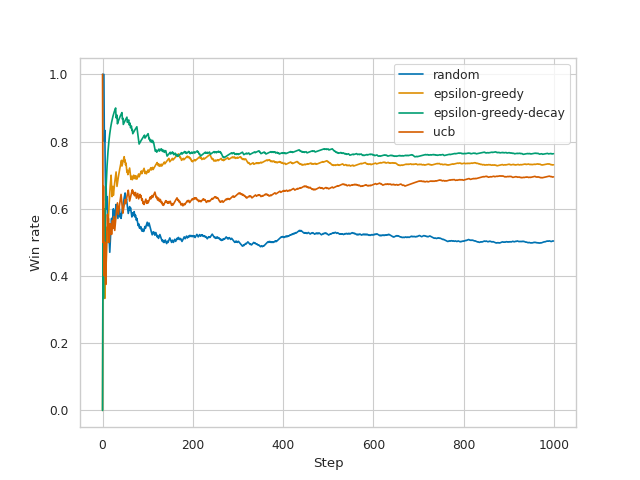
\includegraphics[width = \textwidth]{hw/HW1/bandit_4d1.png}
\end{solution}

\paragraph{For \texttt{bandit\_probs = [0.1, 0.6, 0.4]}.}
\begin{solution}
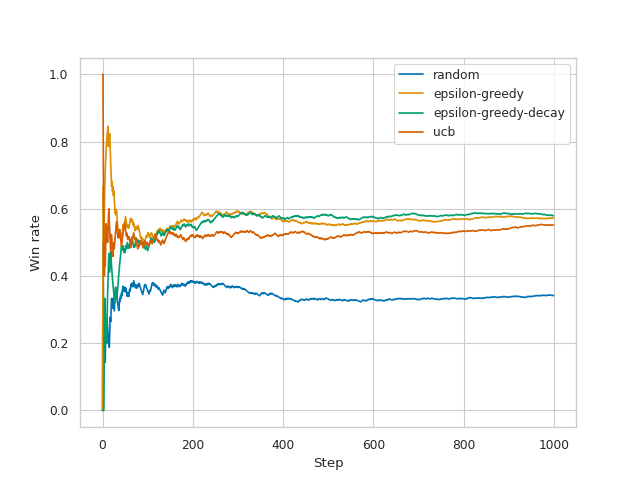
\includegraphics[width = \textwidth]{hw/HW1/bandit_4d2.png}
\end{solution}

\subsection*{Question 4.e (5 points) } 
\paragraph{Reflection and Analysis.}
After running the experiments, reflect on the performance of each strategy.
\begin{solution}
Q: Which strategy achieved the highest cumulative reward? Why do you think this was the case?\\
A: The $\epsilon$-greedy-decay strategy achieved the highest cumulative reward. This is because the strategy decays the $\epsilon$ as the step increases thus maximizes exploitation over exploration in the later stage of the simulation. \\
Q: How did the performance of the epsilon-greedy strategy change with different values of epsilon?\\
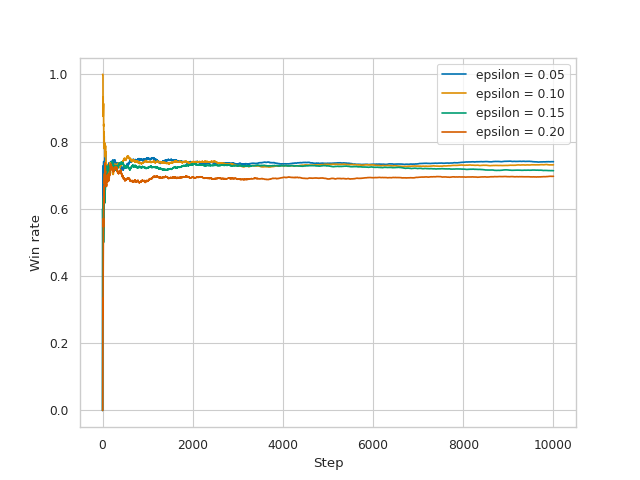
\includegraphics[width = \textwidth]{hw/HW1/bandit_4d3.png}
A: As shown in the plot here, the performance of the epsilon-greedy strategy decreases as epsilon increases. Which means higher rate of exploration is harmful in later stage of the simulation.\\
\end{solution}
\end{document}
